A evolução dos inversores comutados (conversores CC--CA) foi fundamental para viabilizar o avanço das tecnologias de
geração eólica e solar fotovoltaica.
Além da própria evolução tecnológica empregada na fabricação dos dispositivos semicondutores, foi a imposição de uma
limitação para operar os transistores apenas em dois estados --- corte e na saturação --- que possibilitou seu uso no
processamento de potência de forma eficiente.

Idealmente, nesses dois estados, o transistor não apresentaria perdas.
No entanto, essa limitação, embora essencial para lidar com altos níveis de potência, impede que os inversores consigam
impor em sua saída níveis de tensão contínuos, como tensões senoidais.
Essa forma seria desejável para injetar potência na rede (também senoidal).

Um inversor convencional de tensão imposta monofásico geralmente é composto por 4 transistores, cada um operando como uma
chave eletrônica --- aberta ou fechada.
Excluindo algumas combinações que levariam a curto--circuitos e à não imposição da tensão de saída, restam as
4 permutações válidas dos estados desses interruptores que resultam em apenas 3 níveis possíveis de tensão de saída:
positivo ($+V_{dc}$), negativo ($-V_{dc}$) e zero ($0$).

A solução adotada para contornar essa limitação consiste em emular valores intermediários de tensão por meio da
comutação entre esses três níveis válidos.
Controlando-se o tempo de permanência de cada estado ativo, é possível ajustar a tensão média quase instantânea na
saída do conversor.

Ao variar a relação entre os tempos de condução e bloqueio seguindo uma referência senoidal, obtém-se uma forma de onda
comutada que, após filtragem adequada, se aproxima de uma tensão senoidal.
Esse processo é conhecido como modulação.

Além de permitir a síntese de formas de onda que aproximam tensões senoidais, através da modulação
apropriada podemos impor além do formato, a amplitude, frequência e fase da tensão de saída, o que é essenciais
para o controle da energia injetada na rede elétrica.




A \figr{fig:inv} apresenta um circuito simplificado de um inversor monofásico conectado à rede elétrica
convencional, e poderia modelar a interface com a rede em um sistema de geração fotovoltaica.
Esse circuito está dividido em três partes: inversor, que através da lógica de modulação entrega tensão comutada à
saída; um par RL série representando a impedância do filtro de saída
do inversor combinado com a impedância da rede; e uma fonte de tensão, representando a rede de energia como um
barramento infinito.
\begin{figure}[htbp]
    \centering
    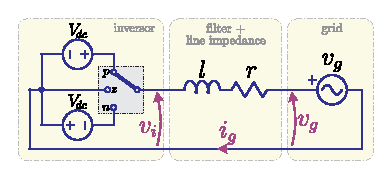
\includegraphics{figs/inv.eps}
    \caption{Modelo de um inversor monofásico conectado à rede elétrica.}
    \label{fig:inv}
\end{figure}

%A tensão da rede é definida por:
%\begin{equation}
%    \label{eq:vg}
%    v_g(t) = \sqrt{2} \cdot V_g \cdot \sin(2 \cdot \pi \cdot f_1 \cdot t)
%\end{equation}
%onde $V_g$ é o valor nominal rms da tensão da rede e $f_1$ sua frequência.

A tensão do inversor ($v_i$) é comutada e possui apenas três níveis: positiva no valor de $V_{dc}$, negativa no valor
de $-V_{dc}$ ou zero.
Quem define o estado instantâneo da tensão do inversor é o modulador, e o faz baseado na comparação de dois sinais
intermediários denominados moduladora ($v_m$) e portadora ($v_c$).
A moduladora representa o sinal que desejamos ter na saída do inversor enquanto a portadora carrega a
informação da frequência de comutação.
Essa técnica é conhecida como modulação por largura de pulso (PWM) senoidal, e é uma das modalidades de modulação mais
simples e empregada em inversores, embora não seja a única.

A moduladora é o sinal que desejamos emular, e pode ser definida por:
%\begin{equation}
%    v_m(t) = \sqrt{2} \cdot V_i \cdot \sin(2 \cdot \pi \cdot  f_1 \cdot t + \varphi_i)
%\end{equation}
%onde $V_i$ é o valor rms que desejamos impor na saída do inversor, $f_1$ sua frequência fundamental (igual da rede no
%caso de um sistema fotovoltáico) e
%$\varphi_i$ a fase da tensão imposta pelo inversor relativa à rede elétrica.
\begin{equation}
    v_m(t) = \sqrt{2} \cdot V_i \cdot \sin(\theta + \varphi_i)
\end{equation}
onde $V_i$ é o valor rms que desejamos impor na saída do inversor, $\theta$ a fase instantânea da rede elétrica e
$\varphi_i$ a fase da tensão imposta pelo inversor relativa à rede elétrica.

A portadora utilizada é um sinal triangular definido por:
\begin{equation}
    \label{eq:c}
    v_c(t) = V_{dc} \cdot \left( 4 \cdot \text{abs}\! \left( \text{mod} (f_c \cdot t, 1) - \tfrac{1}{2} \right)   -1 \right)
\end{equation}
onde $t$ é o tempo,  $V_{dc}$ é a tensão do barramento CC e $f_c$ a frequência da portadora, que definirá a frequência de comutação
dos transistores e, por consequência, a da tensão comutada na saída do inversor.

Finalmente, a tensão do inversor é obtida através de comparações entre a moduladora e a portadora, e é dada por:
\begin{equation}
    \label{eq:vi}
    v_i(t)= V_{dc} \cdot [ s_{p}(t) - s_{n}(t) ]
\end{equation}
sendo:
\begin{equation}
    \label{eq:vp}
    s_{p}(t) =
    \left\{
    \begin{aligned}
        1       & \ \ \ \ \ \ , v_m(t) \geq v_c(t) \\
        0       & \ \ \ \ \ \ , \text{outros casos}
    \end{aligned}
    \right.
\end{equation}
e
\begin{equation}
    \label{eq:vn}
    s_{n}(t) =
    \left\{
    \begin{aligned}
        1       & \ \ \ \ \ \ , v_m(t) \leq -v_c(t) \\
        0       & \ \ \ \ \ \ , \text{outros casos}
    \end{aligned}
    \right.
\end{equation}

%Para uma amostragem temporal de $5~\mu$s
A função de transferência da impedância do filtro e rede pode ser aproximada
por uma equação a diferenças, por:
%\begin{equation}
%    i_g(n) = k_0 \cdot v_i(n) - k_0 \cdot v_g(n) + k_1 \cdot i_g(n-1)
%\end{equation}
%onde $k_0$ e $k_1$ são constantes definidas pela indutância, resistência e frequência de amostragem dos sinais,
%enquanto $(n)$ representa a $n$--ésima amostra dos sinais das tensões e corrente.
\begin{equation}
{i_g}\0 = k_0 \cdot {v_i}\0 - k_0 \cdot {v_g}\0 + k_1 \cdot {i_g}\1
\end{equation}
onde $k_0$ e $k_1$ são constantes definidas pela indutância, resistência e frequência de amostragem dos sinais,
enquanto o índice $n$ representa a $n$--ésima amostra dos sinais das tensões e corrente.


Implemente uma função que simule as correntes resultantes em um sistema fotovoltaico conectado à rede.
Sua assinatura pode ser:
\begin{minted}{custompython}
def inversor(df: pd.DataFrame, Vi: float, phii: float) -> pd.DataFrame:
    # seu código aqui
    return df
\end{minted}

A função recebe como primeiro argumento um \inlcode{DataFrame} contendo as séries temporais \inlstr{time}, \inlstr{phase} e \inlstr{voltage}, que representam,
respectivamente, o tempo ($t$), a fase instantânea da tensão da rede ($\theta$) e a própria tensão da rede
elétrica ($v_g$).

Além disso, a função recebe mais dois parâmetros numéricos: \inlcode{Vi}, correspondente ao valor eficaz da tensão imposta pelo inversor ($V_i$), e \inlcode{phii}, que define a defasagem da tensão de saída do inversor
em relação à fase da rede elétrica ($\varphi_i$).


A função deve resolver as equações de modulação e simulação (eq. a diferenças) e retornar um \inlcode{DataFrame} com as séries:
$t$, $\theta$, $v_g$, $v_m$, $v_c$, $v_i$, $i_g$.

Escreva ainda um scrip que gere um gráfico com esses sinais.

Para o argumento \inlcode{df}, utilize os dados da porção sincronizada das séries de tempo, fase e tensão que foram
geradas e exportadas para um arquivo \colorurl{.csv} na Etapa 3 da questão \inlcode{pll}.

Utilize os seguintes valores para os parâmetros adicionais da função: \inlcode{Vi=250} e \inlcode{phii=0.4}.

Assuma as seguintes constantes, previamente calculadas para a frequência de amostragem do problema:
\begin{equation}
    \label{eq:const}
    \begin{aligned}
        V_{dc} &= 400~\text{V}\\
        f_{c} &= 600~\text{Hz} \\
        k_{0} &=  3.3333 \cdot 10^{-4} \\
        k_{1} &= 0.99963\\
    \end{aligned}
\end{equation}


A \figr{fig:plotsinv} apresenta o resultado esperado:
\begin{figure}[htbp]
    \centering
    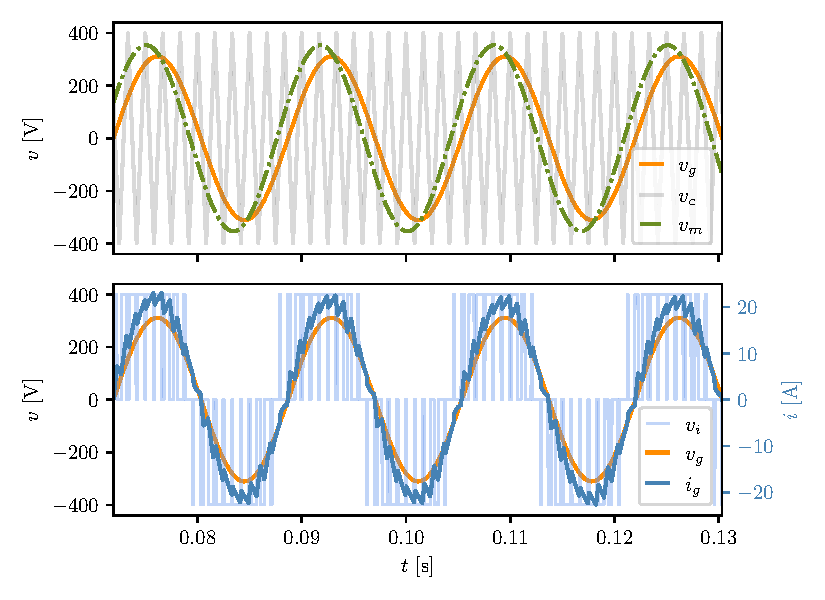
\includegraphics[scale=1.0]{figs/inv1}
    \caption{Resultado gráfico esperado do script.}
    \label{fig:plotsinv}
\end{figure}


%$^\dagger$\emph{Nesta questão foi assumido que o inversor pode impor apenas 3 níveis de tensão, já que é essa a estrutura de inversores de frequência mais
%    simples e difundida. Com o emprego de uma maior quantidade de interruptores controlados, interconectados de forma adequada e com a correta
%    subdivisão do barramento CC, é possível criar variações desse inversor onde o número de níveis permitidos da tensão de saída também é maior.
%    Esses inversores são conhecidos como multiníveis e embora possam apresentar uma grande número de níveis da tensão de saída (o que não é o comum),
%    essa inda manterá sua característica comutada, inerente da imposição de operação dos transistores apenas como interruptores abertos ou fechados.
%    O uso de inversores multiníveis é particularmente interessante em aplicações de média tensão, já que além de criar níveis de tensão
%    intermediários, essas variações possibilitam que cada interruptor eletrônico opere com apenas uma fração da tensão do barramento CC.
%    Nesses caso, as equações \eq{eq:c} e \eq{eq:vi} precisam ser adaptadas.
%}